%---------------------------------------------------------------------------------
% Monte Carlo Simulations
%---------------------------------------------------------------------------------

\section{Monte Carlo Simulations}

\subsection{Approximation of $\pi$}

We will use this toy example as a brief introduction to Monte Carlo Simulations. Lets assume that we are trying to find an approximation for $\pi$. We can still do this using the same randomization-based process as before. We will use the statistical and programming software R for our process. This is a particularly interesting example, as there are very little conditions to actually be satisfied. The only condition that needs to be met as has been said time again is that the sample is representative of the population. In our case, the population is the points $x,y\in\mathscr{R}: x,y\sim U(-0.5,0.5)$. 
\begin{center}
    \begin{lstlisting}[language = R]
        ```{r}
        runs <- 100000
        x <- runif(runs,min=-0.5,max=0.5)
        y <- runif(runs,min=-0.5,max=0.5)
        in.circle <- x^2 + y^2 <= 0.5^2
        mc.pi <- (sum(in.circle)/runs)*4
        ```
    \end{lstlisting}
\end{center}
\newline\\
We've made sure that that $x$ and $y$ are representative of each population by selecting a random value from $U(-0.5,0.5)$ using the \textbf{runif()} command which stands for "random uniform". Rather than a least squares estimator, in this case, our test statistic will be the Bernoulli random variable representing whether a point is contained within the circle which inscribes our population distribution. Now that we have our test statistics, we can approximate $\pi$. Empirically, $A_{square}=(2r)^2=4r^2$. Suppose we don't know a value for $\pi$, but instead know that $A_{circle}\propto r^2$. That is, $A_{circle}=cr^2$ where $c$ is a positive constant. We can now approximate $\pi$ where $c$ is our approximation. This is as simple as taking the proportion of $A_{circle}$ and $A_{square}$.

$$
\frac{A_{circle}}{A_{square}} = \frac{cr^2}{4r^2} = \frac{c}{4}\longrightarrow\frac{4\cdot A_{circle}}{A_{square}}
$$
\\
The simulated $A_{circle}$ that we have is just the total number of points inside of the circle while $A_{square}$ will be the total number of points that we sampled. The approximation for $\pi$ in this example is $3.14252$, not too far off from the true value of $3.14159$.

\begin{figure}[htpb!] % Defines figure environment
    \centering % Centers your figure
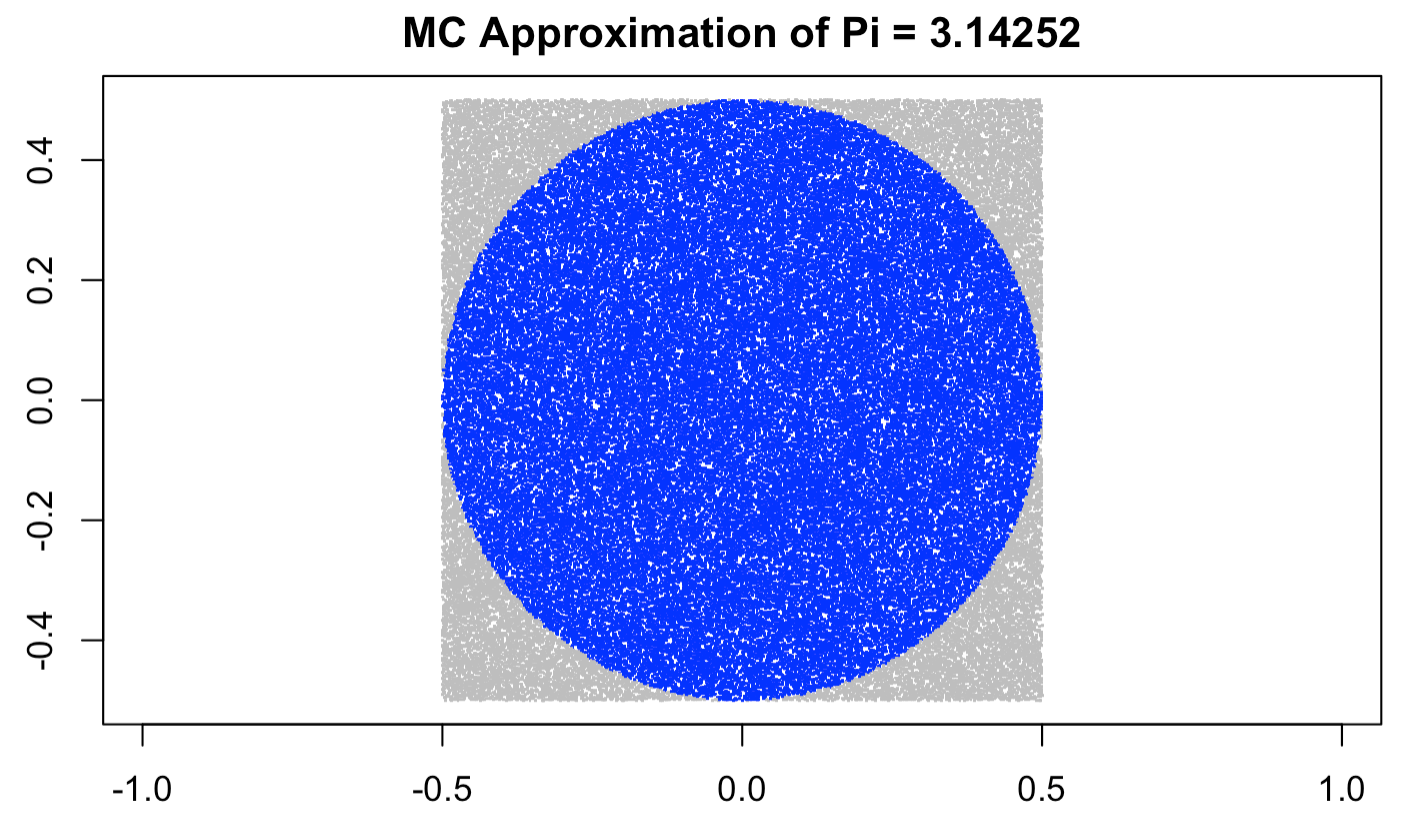
\includegraphics[scale=0.4]{figure/monteCarloCircle.png} % Includes your figure and defines the size
    \caption{Plot of sampling distribution and inscribed circle} % For your caption
    \label{fig:my_label} % If you want to label your figure for in-text references
\end{figure}

\subsection{Monte Carlo Simulation and RBI}

The Monte Carlo simulation is a do-it-all kind of method which has many useful applications in statistics and mathematics in general. For randomization based inference, Monte Carlo simulations manifest themselves as a streamlined way to get the asymptotically correct p-value we want. The process is applied as follows: First, instead of taking $n!$ permutations of our data, we take a random sample of permutations usually between 5 to 100. We then calculate the proportion of those permutations that yield a test statistics that are as or more extreme than our original test statistic. Now we have our random variable $P$ (the aforementioned proportion) with which we create a 95\% confidence interval using the largest possible binomial standard deviation, $\sqrt{n*(0.5)(1-0.5)}$. Thus, we create a sufficiently wide confidence interval that, if created over and over again, will contain the true p-value for our effect 95\% of the time. 
